\documentclass[tikz,border=5mm]{standalone}
\usepackage{pgfplots}
\usepackage{amsmath}
\pgfplotsset{compat=1.18}

\definecolor{planebg}{RGB}{120, 195, 205}
\definecolor{triedge}{RGB}{0, 50, 220}
\definecolor{normgreen}{RGB}{0, 110, 20}
\definecolor{dotred}{RGB}{204, 30, 30}

\begin{document}
	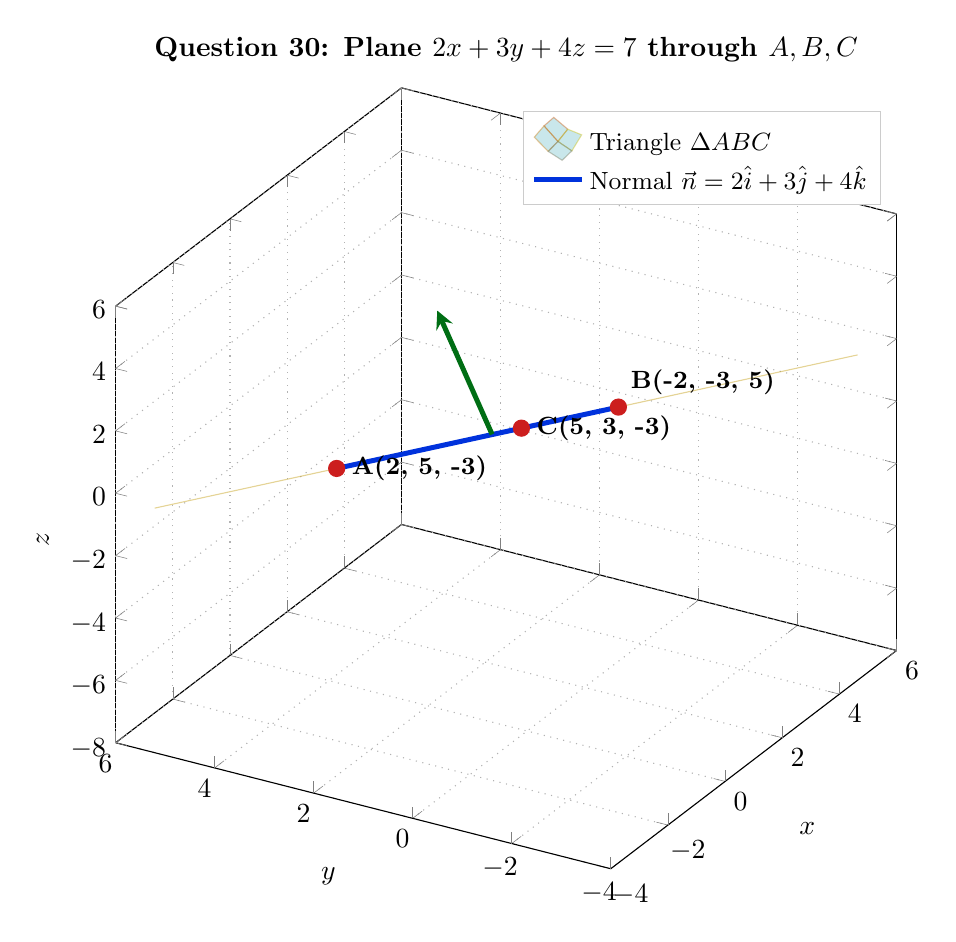
\begin{tikzpicture}
		\begin{axis}[
			width=11.5cm, height=11.5cm,
			view={-60}{30},
			title={\textbf{Question 30: Plane $2x + 3y + 4z = 7$ through $A, B, C$}},
			xlabel={$x$}, ylabel={$y$}, zlabel={$z$},
			xmin=-4, xmax=6,
			ymin=-4, ymax=6,
			zmin=-8, zmax=6,
			xtick={-4, -2, 0, 2, 4, 6},
			ytick={-4, -2, 0, 2, 4, 6},
			ztick={-8, -6, -4, -2, 0, 2, 4, 6},
			grid=both,
			grid style={dotted, gray!60},
			legend cell align={left},
			legend style={at={(0.98,0.97)}, anchor=north east, font=\small, draw=gray!40}
			]
			% Plane surface patch 2x + 3y + 4z = 7  =>  z = (7 - 2x - 3y)/4
			\addplot3[
			surf, opacity=0.4, fill=planebg, draw=none,
			domain=-3.5:5.5, domain y=-3.5:5.5, samples=2
			] {(7 - 2*x - 3*y)/4};
			
			% Triangle ABC edges
			\addplot3[triedge, line width=1.8pt] coordinates {
				(2, 5, -3) (-2, -3, 5) (5, 3, -3) (2, 5, -3)
			};
			\addlegendentry{Triangle $\Delta ABC$}
			
			% Normal Vector: n = 2i + 3j + 4k (originating from plane centroid)
			\addplot3[normgreen, line width=1.8pt, -{stealth[scale=1.3]}] coordinates {
				(1.67, 1.67, -0.33) (2.87, 3.47, 2.07)
			};
			\addlegendentry{Normal $\vec{n} = 2\hat{i} + 3\hat{j} + 4\hat{k}$}
			
			% Vertex points and labels
			\node[circle, fill=dotred, inner sep=2.2pt] at (axis cs:2, 5, -3) {};
			\node[right=2pt, font=\small\bfseries] at (axis cs:2, 5, -3) {A(2, 5, -3)};
			
			\node[circle, fill=dotred, inner sep=2.2pt] at (axis cs:-2, -3, 5) {};
			\node[above right=1pt, font=\small\bfseries] at (axis cs:-2, -3, 5) {B(-2, -3, 5)};
			
			\node[circle, fill=dotred, inner sep=2.2pt] at (axis cs:5, 3, -3) {};
			\node[right=2pt, font=\small\bfseries] at (axis cs:5, 3, -3) {C(5, 3, -3)};
		\end{axis}
	\end{tikzpicture}
\end{document}